\documentclass{beamer}

\usepackage{beamer_tom}
\graphicspath{{/home/tom/Pictures/People/}{./images/}{./}}


\usepackage{tikz}
\usepgflibrary{shapes.arrows}

\def\biblio{
    \nobibliography{../../library}
    \def\biblio{}
}

\institute{}
\author{P. Rodrigues, {\bf T. Moreau}, G. Louppe, A. Gramfort}
\title{
    HNPE: Leveraging Global Parameters for Neural Posterior Estimation
    }

    \def\jointwork{
        \includegraphics[height=5em]{prodriguez}
        \hskip5ex
        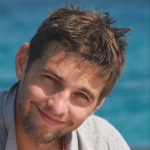
\includegraphics[height=5em]{tommoral}
        \hskip5ex
        \includegraphics[height=5em]{gloupe}
        \hskip5ex
        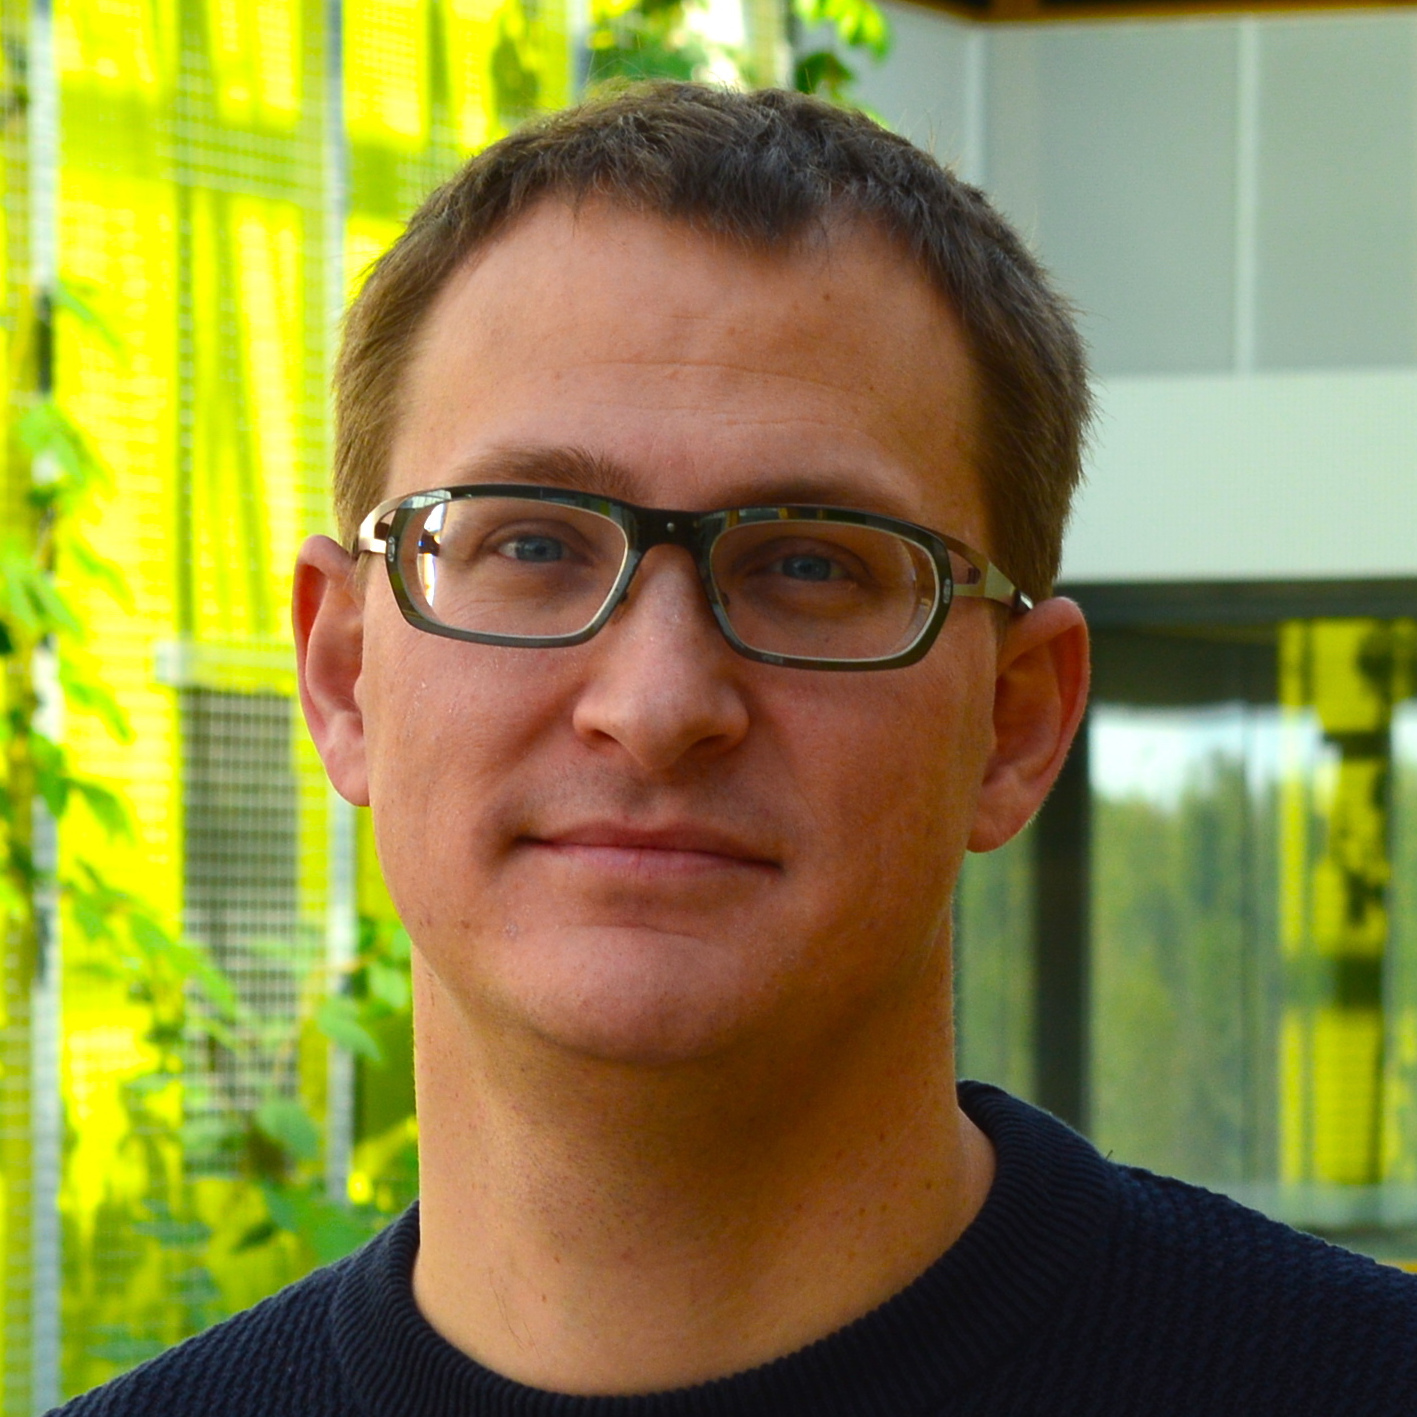
\includegraphics[height=5em]{agramfort}
        \vskip-2.5em
        }

        \setbeamertemplate{title page}[frame]
        \def\extraLogo{}


        \definecolor{palegreen}{RGB}{236,240,241}
        \setbeamercolor{forward}{fg=gray,bg=gray}
        \setbeamercolor{bgcolor}{fg=black!60,bg=palegreen}
        \setbeamercolor{bordercolor}{fg=black!80,bg=darkblue}

\begin{document}
\tikzstyle{forward} = [draw=gray, very thick, single arrow, minimum height=3.2cm, shape border rotate =#1, fill=gray!10]
\tikzstyle{inverse} = [draw=darkred, very thick, single arrow, minimum height=3.2cm, shape border rotate =#1, fill=gray!10]

    \begin{frame}
        \titlepage
    %	\biblio{}
    \end{frame}

    \begin{frame}{Inverse problems}
        \begin{beamercolorbox}[wd=\textwidth, center, sep=.3ex]{separation line}
        \begin{beamercolorbox}[wd=.99\textwidth, center, sep=1ex]{headline}
            Inferring parameters of a model from observations is\\
            a fundamental scientific challenge.
        \end{beamercolorbox}
        \end{beamercolorbox}

        \begin{columns}[T]
            \column{.16\textwidth}
            \column{.32\textwidth}
            Ion channel parameters\\
            \emph{e.g.} conductance.\\[.3em]
            \begin{beamercolorbox}[wd=\textwidth, center, sep=1ex]{bgcolor}
                Hodgkin-Huxley model\\[.3em]
                (neuroscience)
            \end{beamercolorbox}
            Membrane potential

            \column{.32\textwidth}
            Epidemy parameters\\
            \emph{e.g.} $R_0$.\\[.3em]
            \begin{beamercolorbox}[wd=\textwidth, center, sep=1ex]{bgcolor}
                \vskip.5em
                SIR model\\
                (epidemiology)
                \vskip.5em
            \end{beamercolorbox}
            Number of infections

            \column{.16\textwidth}
        \end{columns}
        \vskip1em
        \begin{columns}[T]
            \column{.2\textwidth}
            \vskip2.2em
            \flushright%
            Parameters $\theta$%
            \column{.3\textwidth}
            \begin{beamercolorbox}[wd=\textwidth, center, sep=.3ex]{forward}
            \begin{beamercolorbox}[wd=.97\textwidth, center, sep=1ex]{bgcolor}
                Forward model $\mathcal M$\\
                $\rightarrow$
            \end{beamercolorbox}
        \end{beamercolorbox}
            \begin{beamercolorbox}[wd=\textwidth, center, sep=.3ex]{separation line}
            \begin{beamercolorbox}[wd=.97\textwidth, center, sep=1ex]{block title}
                Inverse model\\
                $\mathbf{\leftarrow}$
            \end{beamercolorbox}
        \end{beamercolorbox}
            \column{.2\textwidth}
            \vskip2.2em
            Observations $x$
            \column{.3\textwidth}
            \visible<2>{
            \centering
            \vskip2em
            {\bf Goal:}\\Learn
            $p(\theta | x)$\\}
        \end{columns}



        \begin{tikzpicture}[overlay]
            \node at (1,4) [forward=-180] {\rotatebox{90}{Forward Model}};
            \node at (11,4) [inverse=90] {\rotatebox{-90}{Inverse problem}};
            \end{tikzpicture}
    \end{frame}

    \begin{frame}
        \frametitle{Key challenge: Non-injective models}

        \begin{columns}
            \column{.25\textwidth}
            \visible<2>{
                \begin{beamercolorbox}[wd=\textwidth, center, sep=.3ex]{bordercolor}
                    \begin{beamercolorbox}[wd=.965\textwidth, center, sep=1ex]{darkbluebox}
                        Other speakers at same distance
                    \end{beamercolorbox}
                \end{beamercolorbox}
            }
            \column{.25\textwidth}
                \centering
                Voice Amplitude
                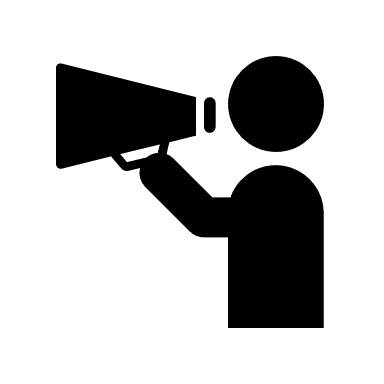
\includegraphics[width=.5\textwidth]{speaker}
            \column{.25\textwidth}
                \centering
                Distance
                
\includegraphics[width=\textwidth]{arrow}
            \column{.25\textwidth}
                \centering
                
\includegraphics[width=.5\textwidth]{mic}\\
        \end{columns}

        \begin{beamercolorbox}[wd=\textwidth, center, sep=.3ex]{separation line}
            \begin{beamercolorbox}[wd=.99\textwidth, center, sep=1ex]{headline}
                Close and quiet or far and loud?
            \end{beamercolorbox}
        \end{beamercolorbox}

        \begin{columns}
            \column{.25\textwidth}
            \visible<2>{
                \begin{beamercolorbox}[wd=\textwidth, center, sep=.3ex]{bordercolor}
                    \begin{beamercolorbox}[wd=.965\textwidth, center, sep=1ex]{darkbluebox}
                        Other recordings from the same subject
                    \end{beamercolorbox}
                \end{beamercolorbox}
            }
            \column{.25\textwidth}
                \centering
                brain activity
                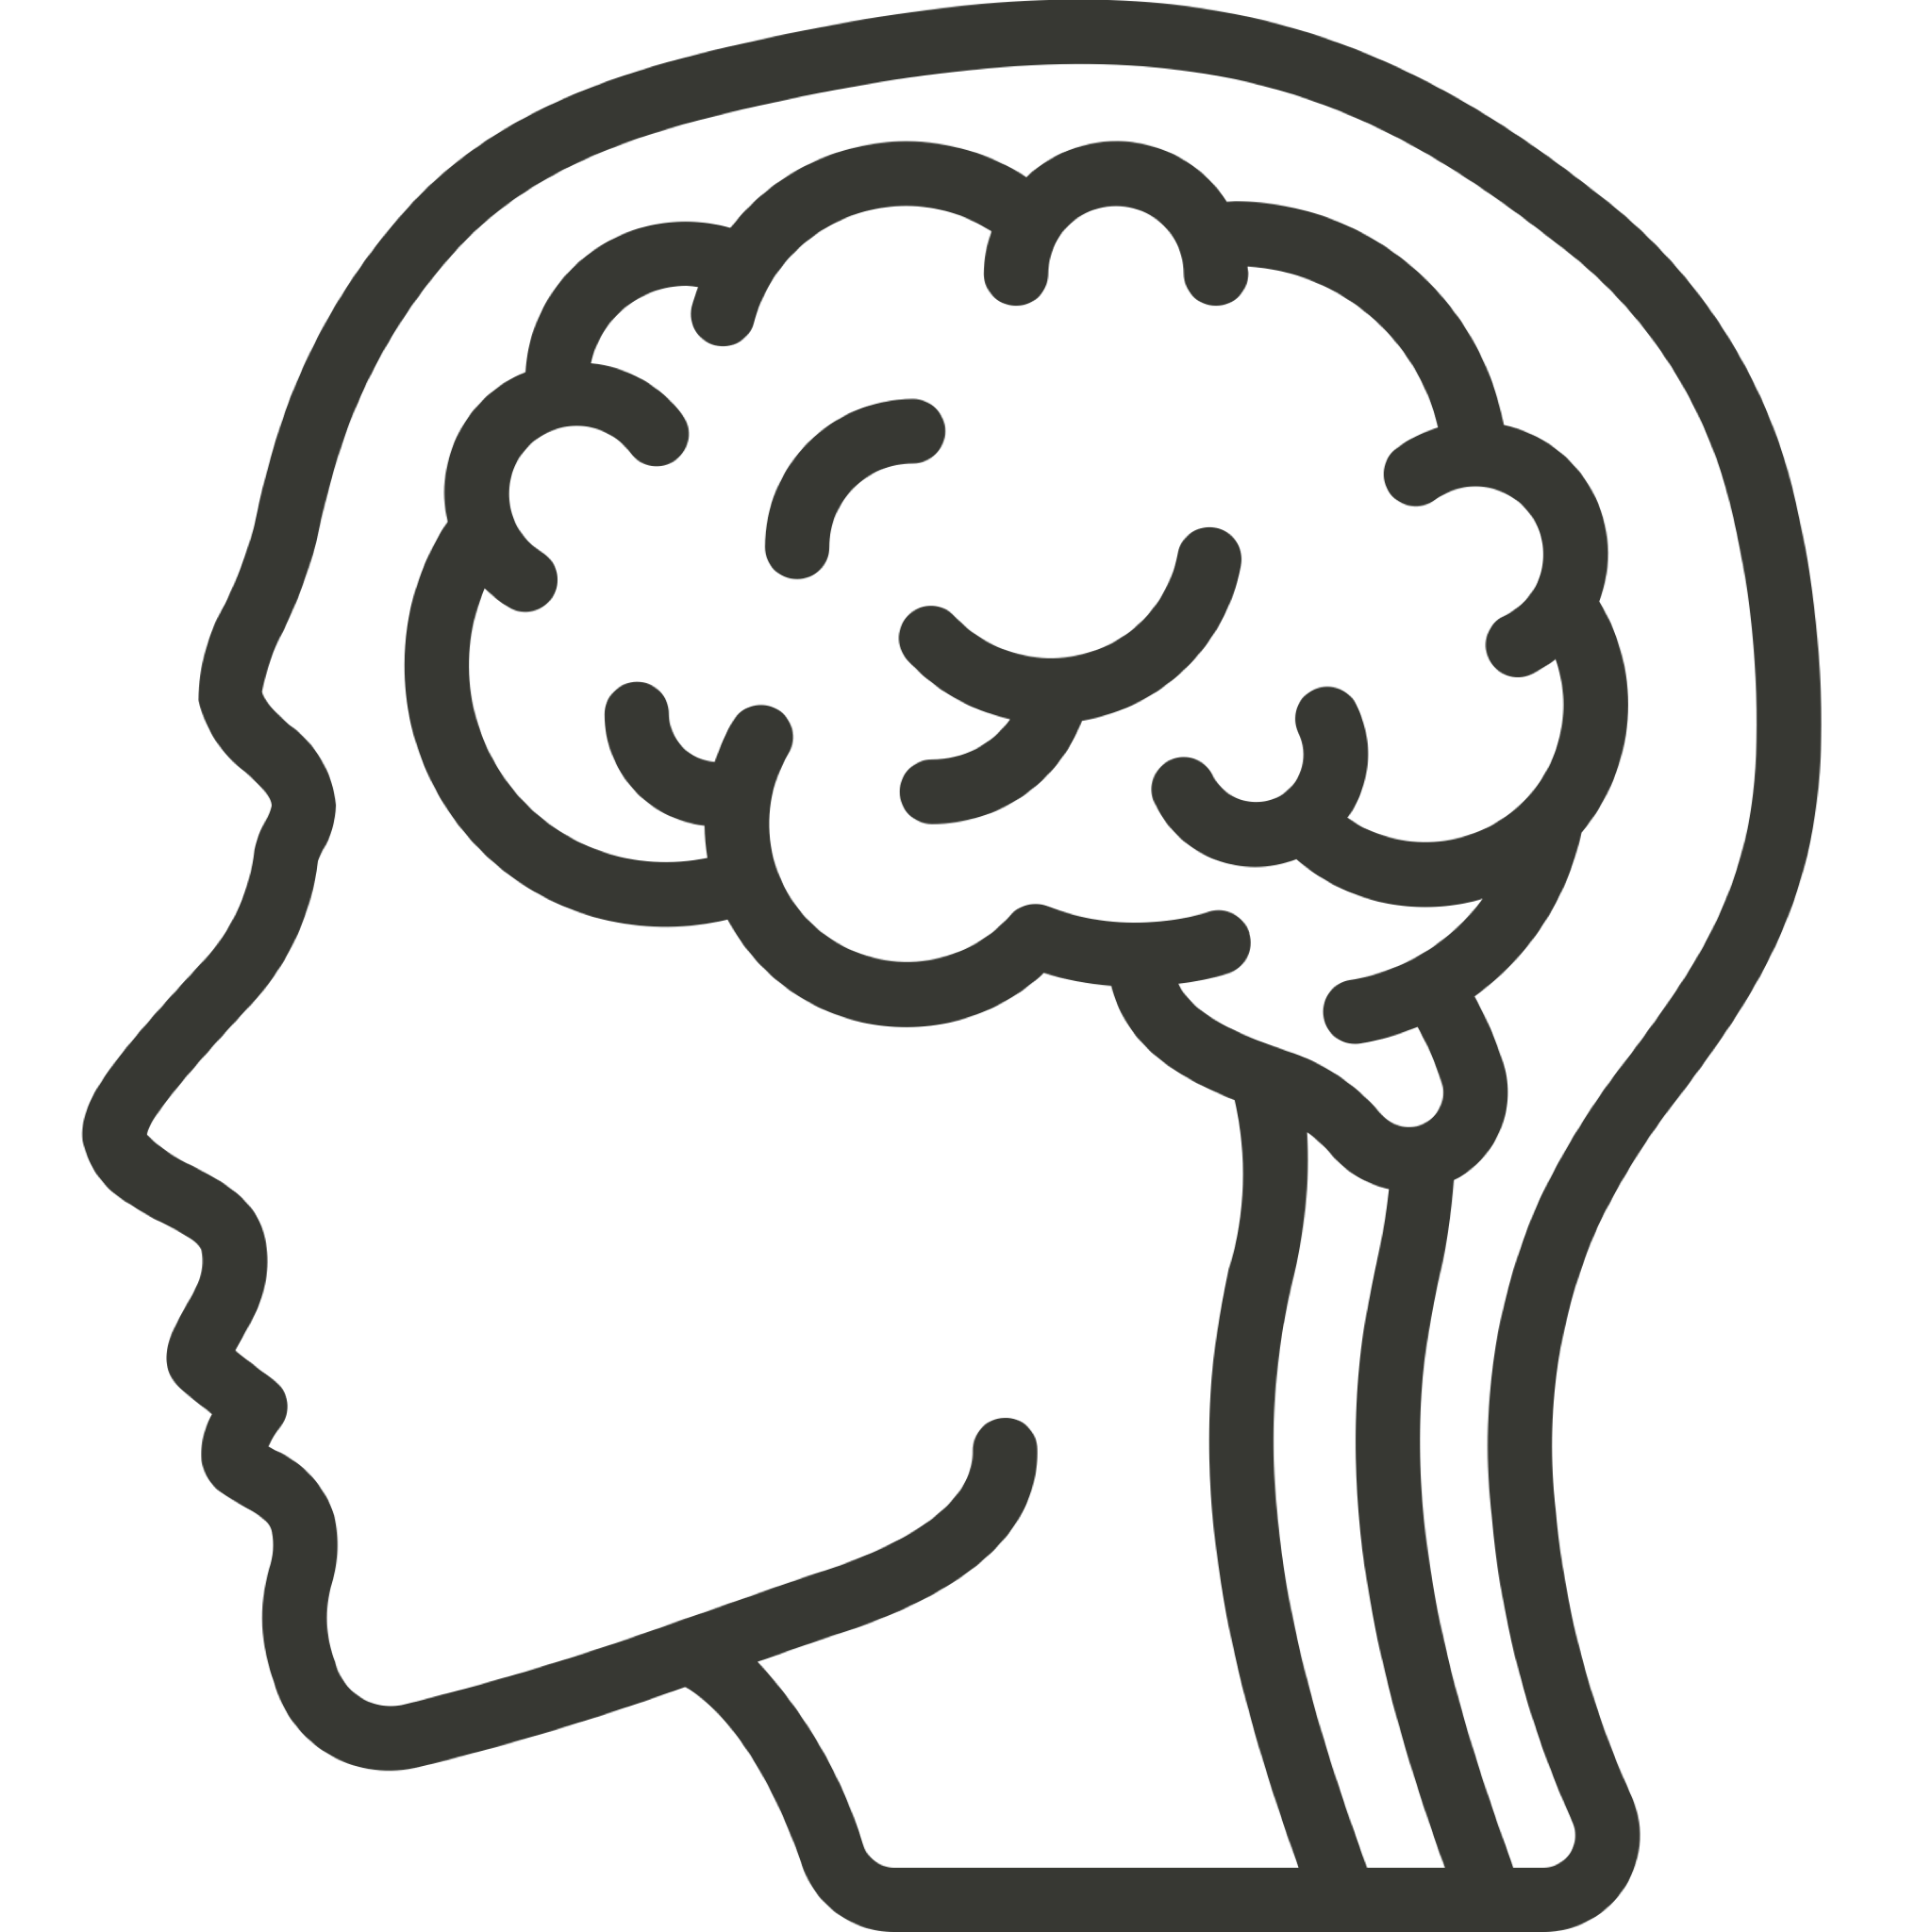
\includegraphics[width=.5\textwidth]{brain}\\
            \column{.25\textwidth}
                \centering
                Brain tissue\\
                
\includegraphics[width=\textwidth]{arrow}\\
                propagation
            \column{.25\textwidth}
                \centering
                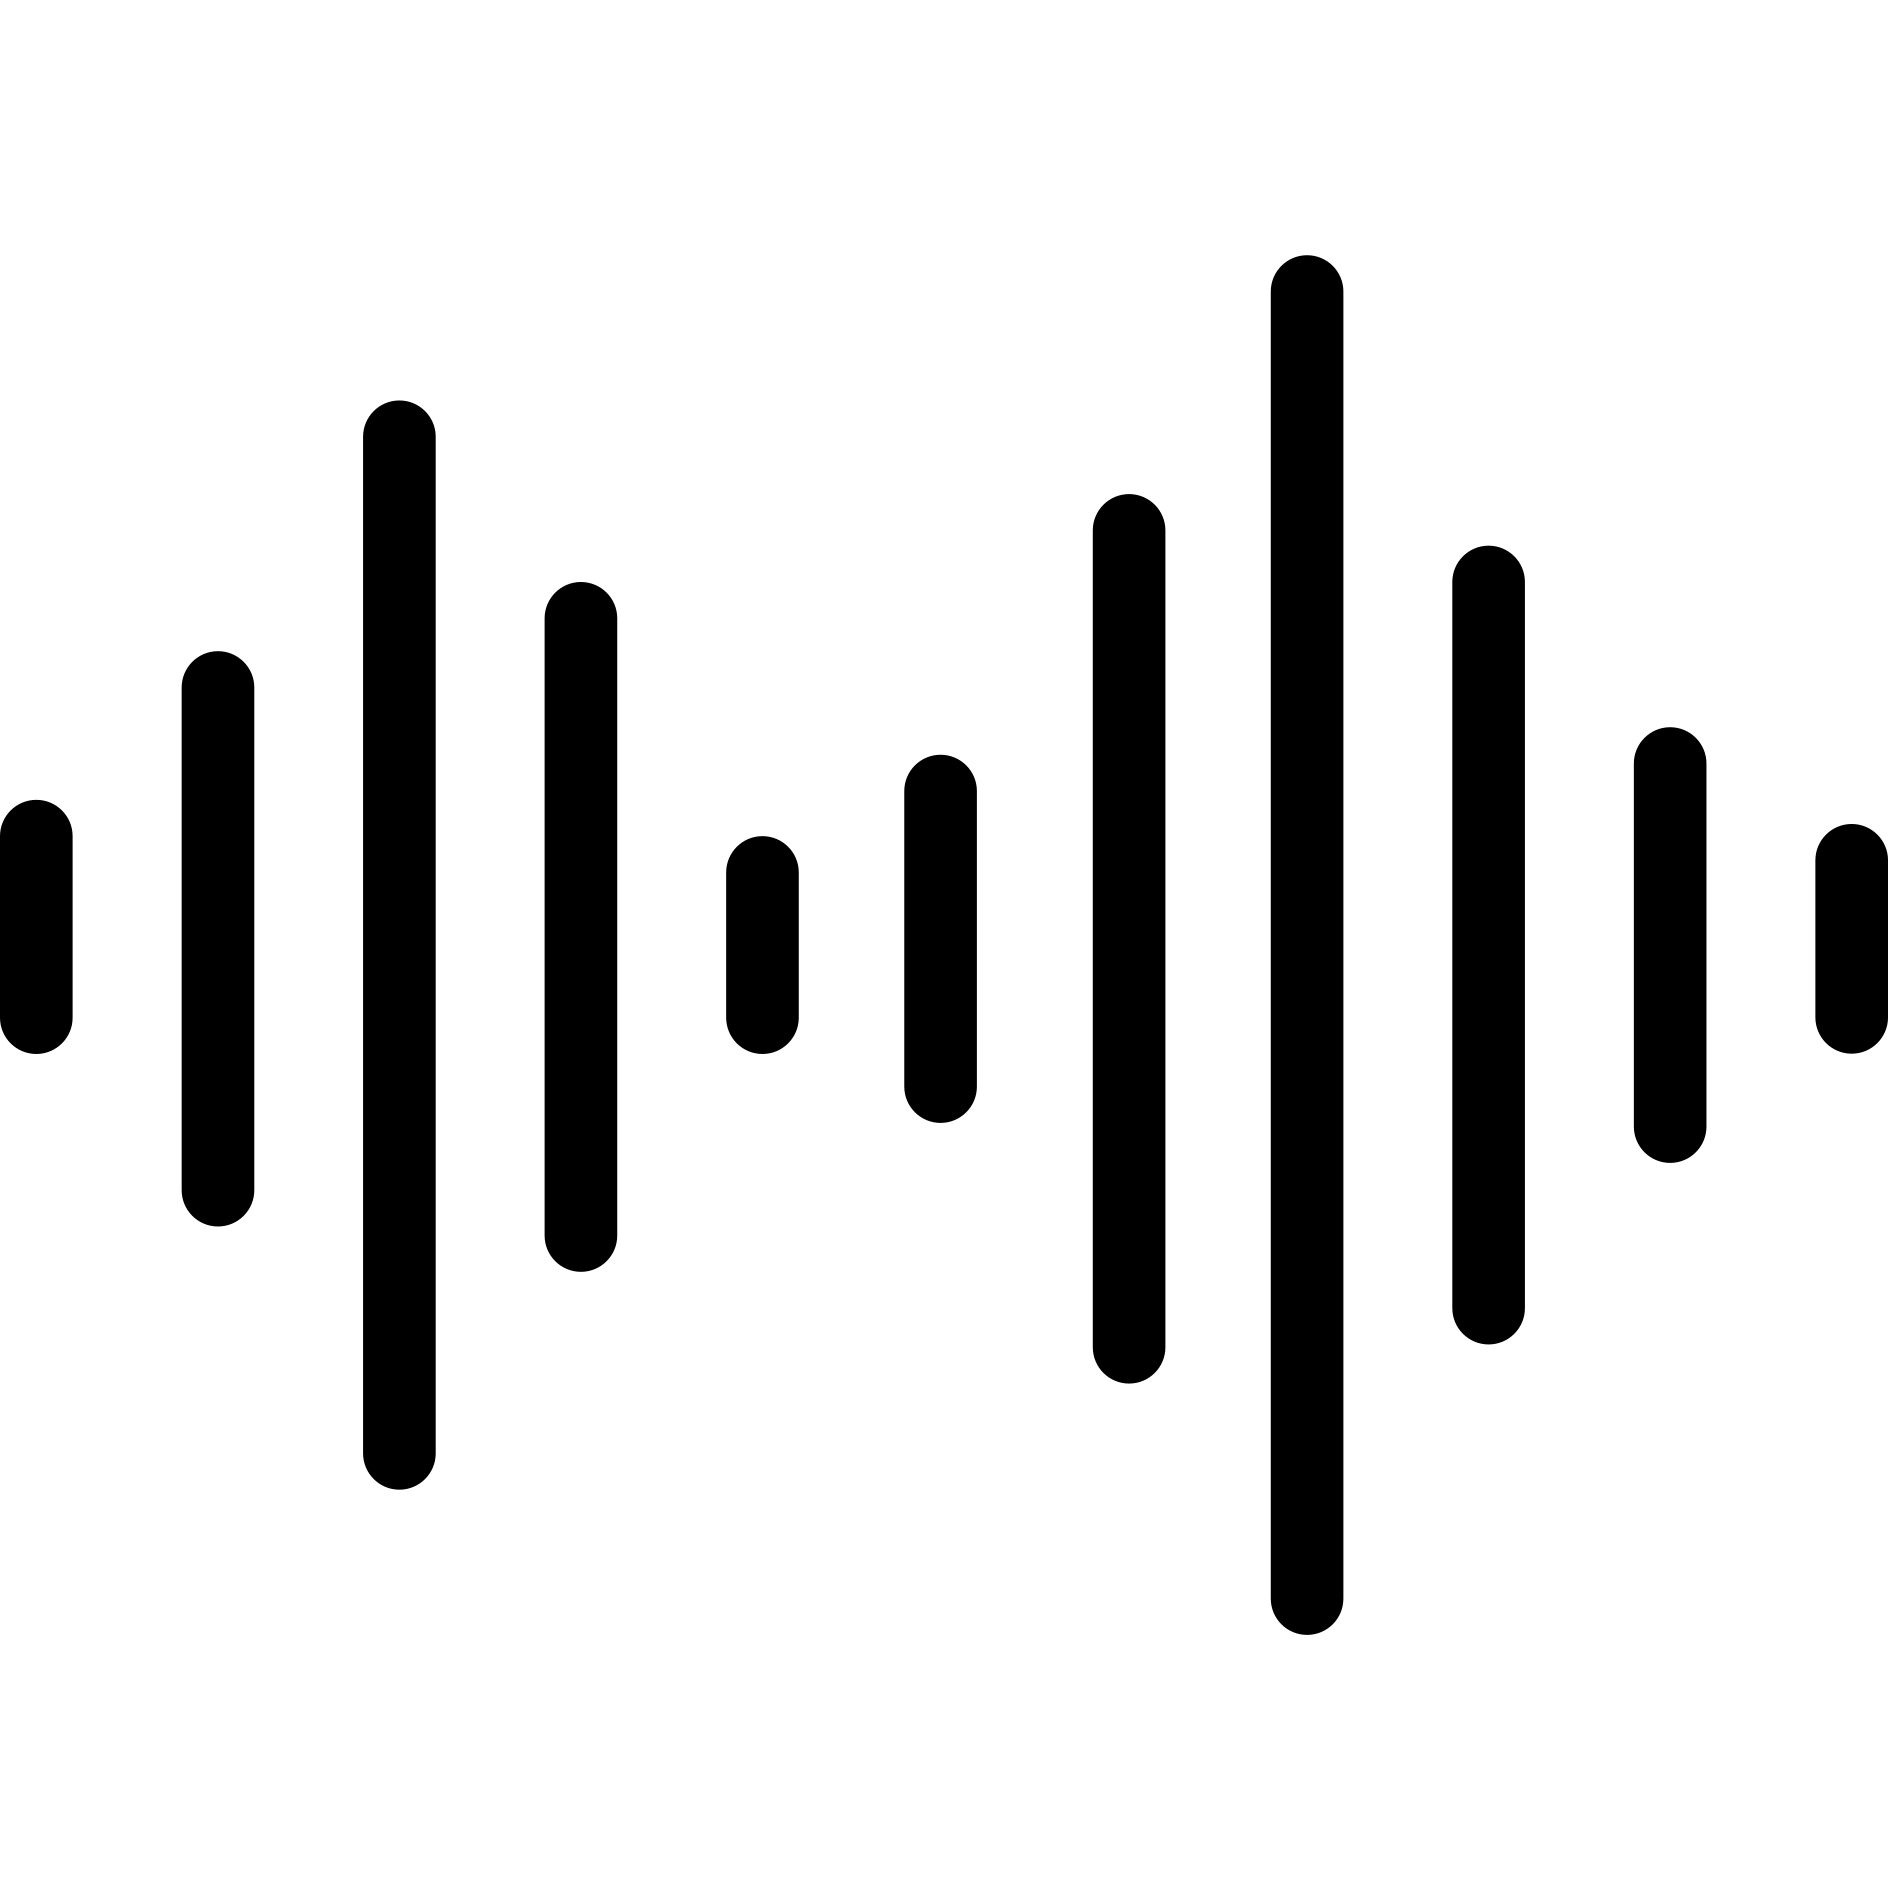
\includegraphics[height=5em]{MEG_signals}
                \vskip-2em\hskip2ex
                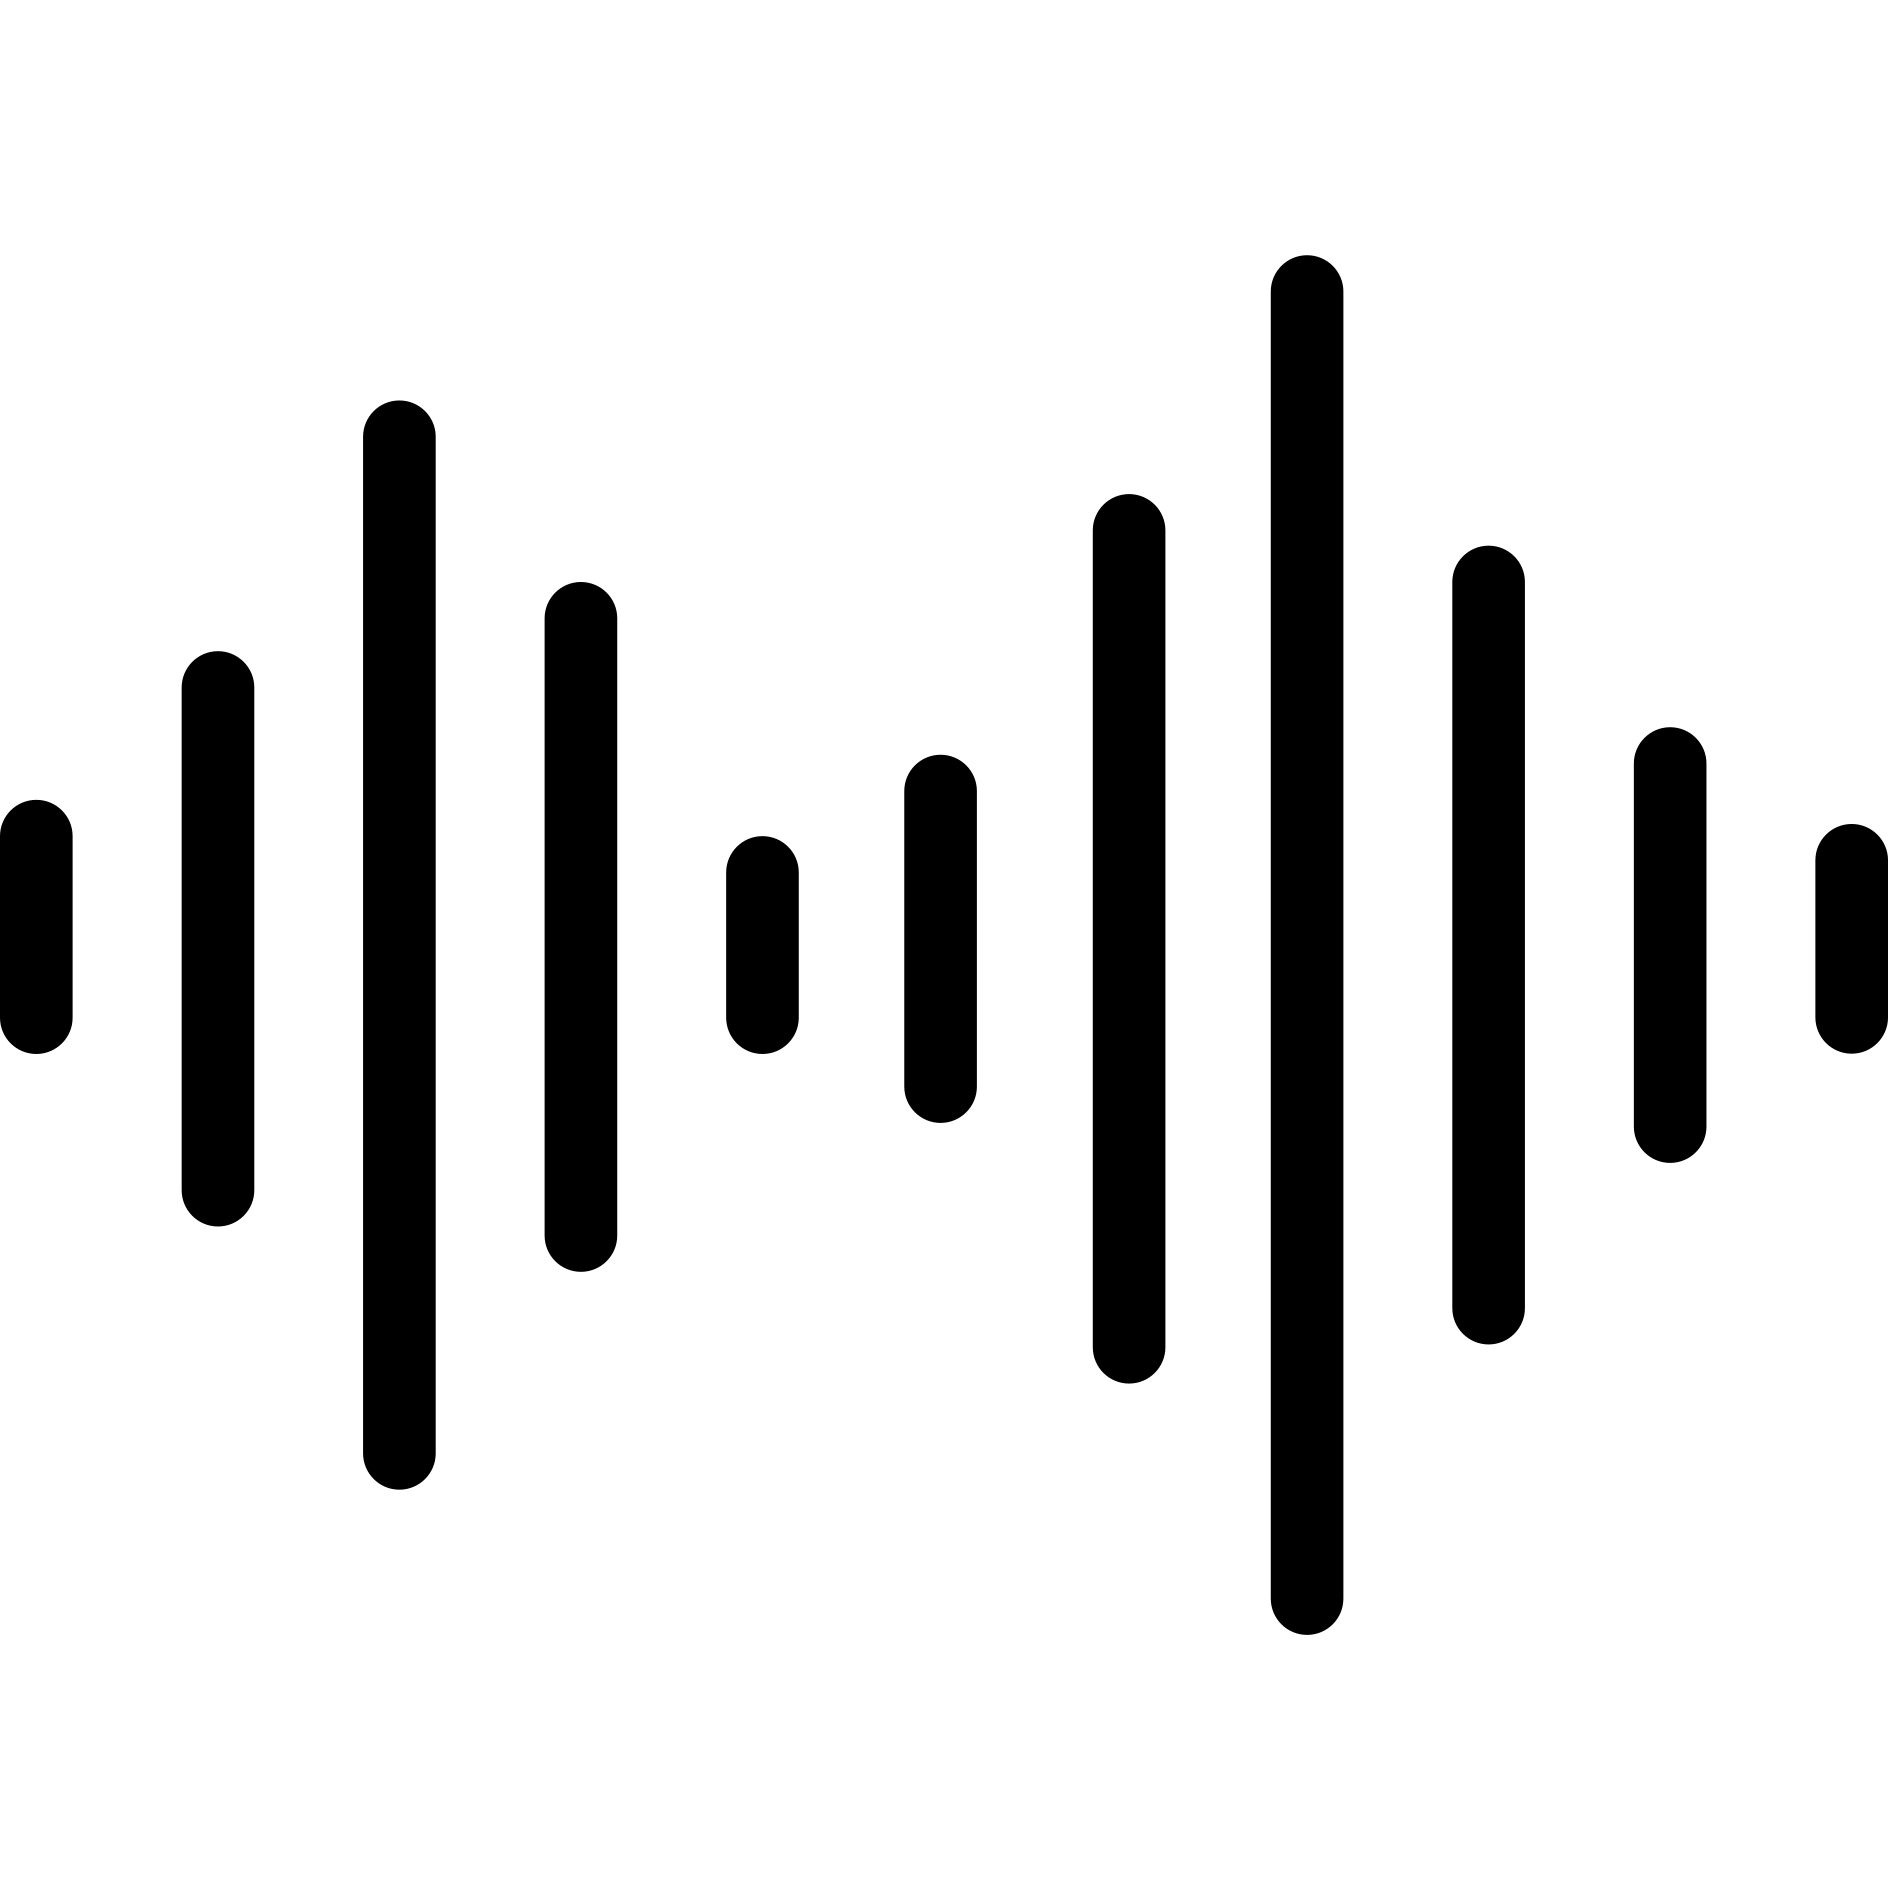
\includegraphics[height=5em]{MEG_signals}
        \end{columns}
        \begin{beamercolorbox}[wd=\textwidth, center, sep=.3ex]{separation line}
            \begin{beamercolorbox}[wd=.99\textwidth, center, sep=1ex]{headline}
                Amplified weak or attenuated strong ?
            \end{beamercolorbox}
        \end{beamercolorbox}
        \visible<2>{
        \strongpoint{Leverage observations with common \emph{global} parameter.}
        }
    \end{frame}

    \frame{
        \frametitle{Our contributions}
        \begin{itemize}\itemsep2em
            \item Hierarchical model to account for extra observations $\mathcal X=\{x_1, \dots x_N\}$,\\
            \item Adapt normalizing flows to approximate the posterior,\\
            \keypoint{[Papamakarios et al. 2019]}
            \item Use DeepSet architecture to account for invariance in $\mathcal X$,\\
            \keypoint{[Zaheer et al. 2017]}
            \item Show its capability on a toy problem and a real neuroscience model.
        \end{itemize}
    }

    \frame{
        \frametitle{Results: Jansen \& Rit Neural Mass Model}

        \begin{columns}

        \column{.3\textwidth}
            \myitem{} Observations $x$ are EEG signals.\\[2em]
            \myitem{} $\theta$ are physiological properties of the brain.
        \column{.7\textwidth}
            {\centering
            \alt<2->{
                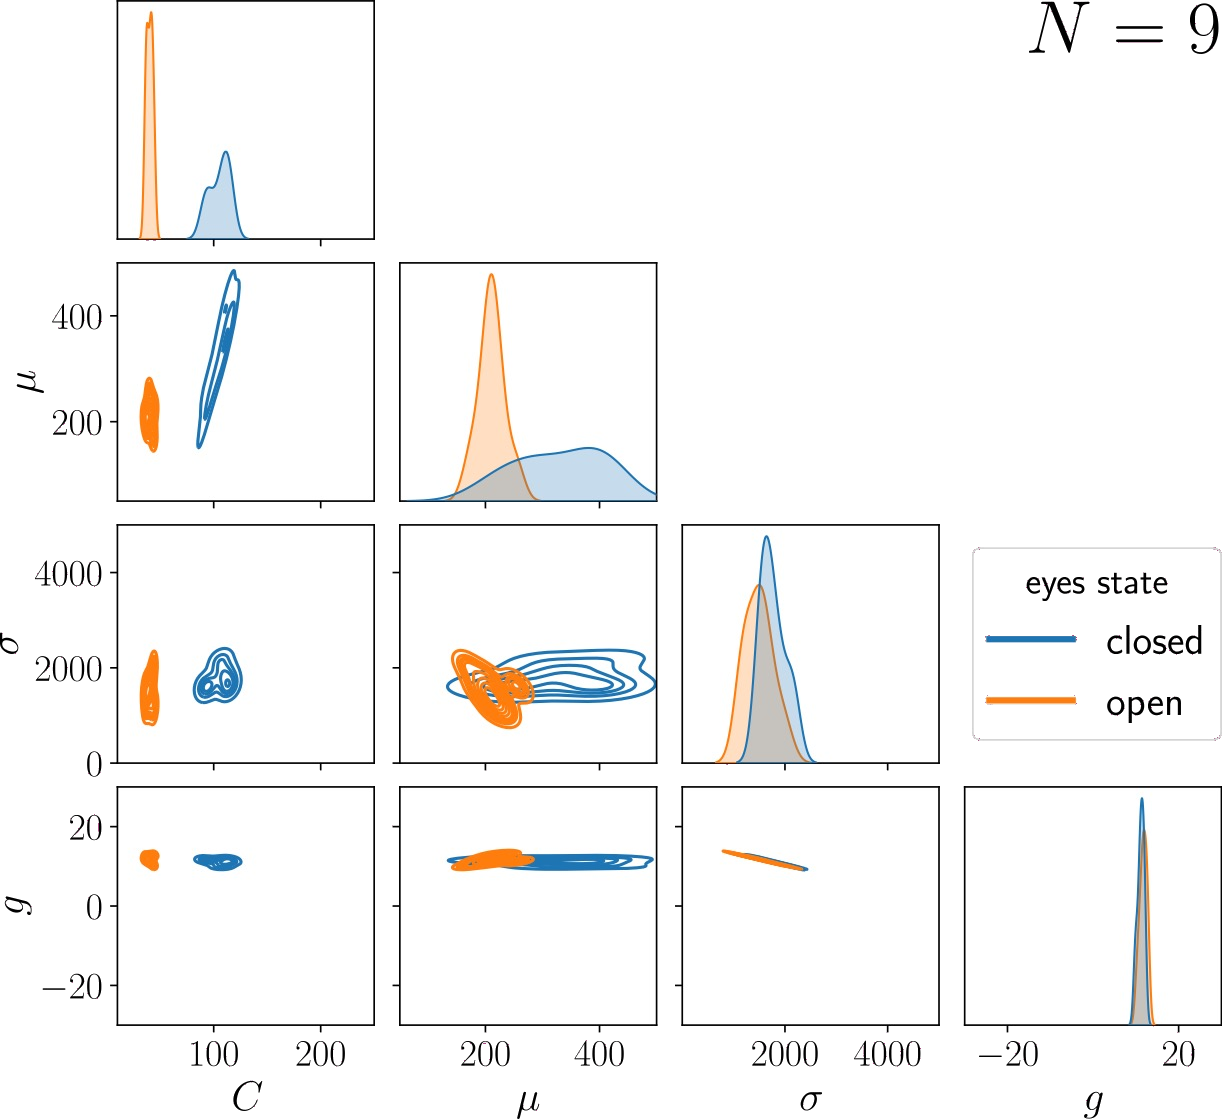
\includegraphics[height=.8\textheight]{alpha_rythm_params}\\
            }{
                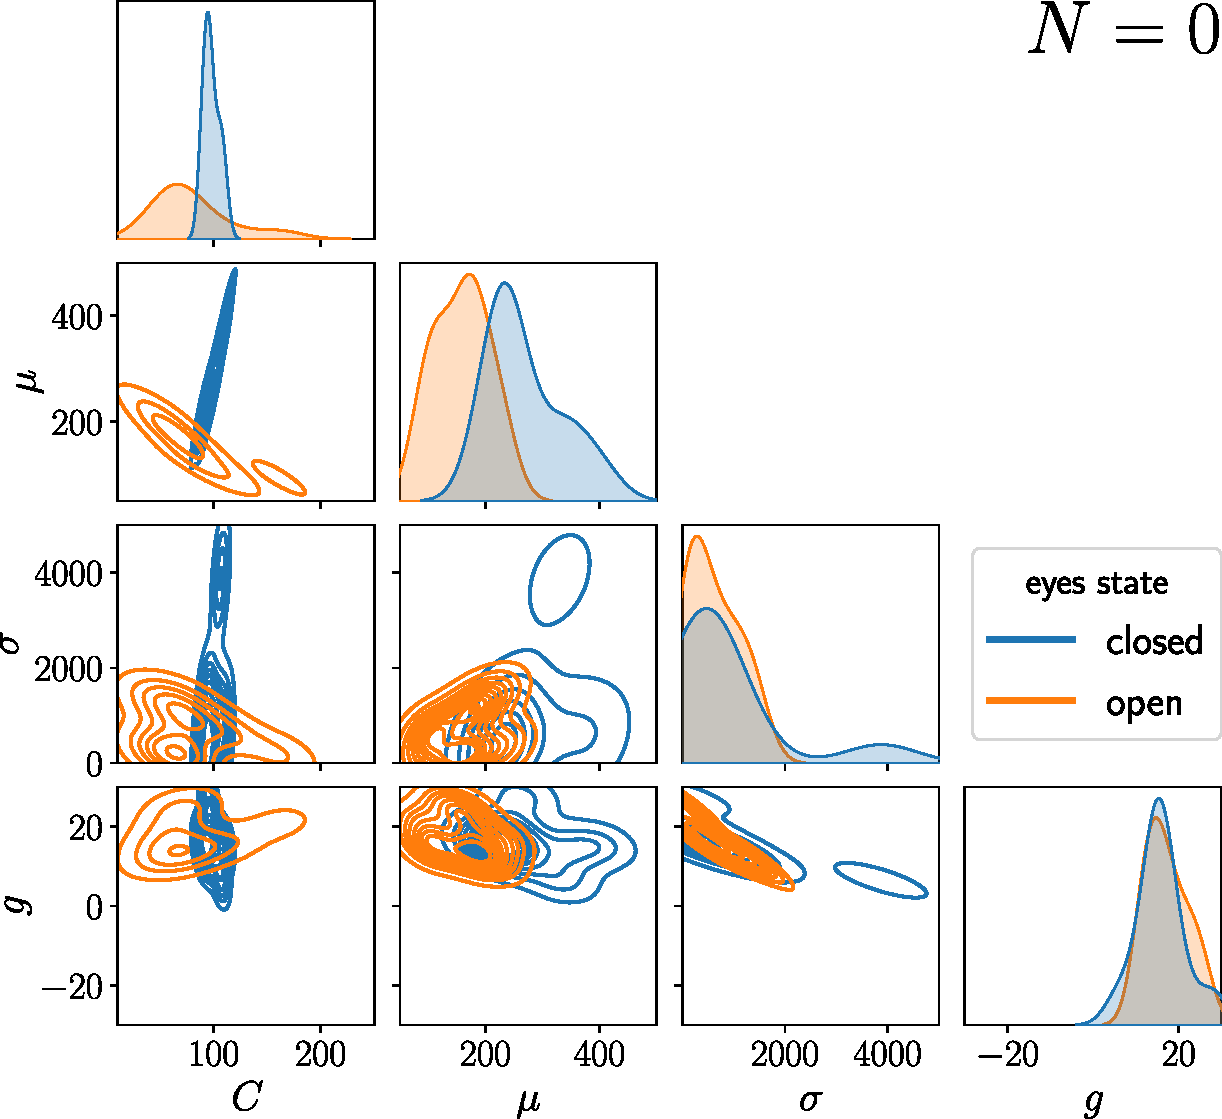
\includegraphics[height=.8\textheight]{JRNMM_real_nextra_0.pdf}\\
            }}
        \end{columns}
    }

    \begin{frame}
        \titlepage
    %	\biblio{}
        {\Large \centering Come visit our poster for more details!\\}
    \end{frame}

\end{document}